\documentclass[border=10pt]{standalone}
\usepackage[T1]{fontenc}
\usepackage[default]{sourcesanspro}
\usepackage{tikz}
\usepackage{fontawesome5}
\usepackage{xcolor}
\definecolor{ForestGreen}{RGB}{34,139,34}
\definecolor{RoyalBlue}{RGB}{65,105,225}
\definecolor{OrangeRed}{RGB}{255,69,0}
\definecolor{Crimson}{RGB}{220,20,60}
\usetikzlibrary{arrows.meta,positioning,fit}

\begin{document}
\begin{tikzpicture}[
            >=Stealth,
            host/.style={rectangle, draw=ForestGreen, fill=ForestGreen!10, rounded corners, minimum width=2.6cm, minimum height=1cm, align=center, font=\small},
            sw/.style={rectangle, draw=RoyalBlue, fill=RoyalBlue!12, rounded corners, minimum width=1.8cm, minimum height=0.9cm, align=center, font=\small},
            router/.style={rectangle, rounded corners, draw=OrangeRed, fill=OrangeRed!12, minimum size=1.2cm, align=center, font=\small},
            netlabel/.style={font=\small\bfseries},
            link/.style={thick}
        ]

        % horizontal column separation
        \def\colsep{3.2}

        % Left LAN (LAN A)
        \node[host] (A1) at ({0*\colsep},1.2) {\faLaptop\\\texttt{192.168.1.10}};
        \node[host] (A2) at ({0*\colsep},0)   {\faLaptop\\\texttt{192.168.1.11}};
        \node[host] (A3) at ({0*\colsep},-1.2){\faLaptop\\\texttt{192.168.1.12}};
        \node[sw]   (SWL) at ({1*\colsep},-0.1) {\faNetworkWired\\Switch};

        % Router between switches
        \node[router] (R) at ({2*\colsep},0) {\faServer\\Router\\\small \texttt{192.168.1.1} \\ \small \texttt{192.168.2.1}};

        % Right LAN (LAN B)
        \node[sw]   (SWR) at ({3*\colsep},-0.1) {\faNetworkWired\\Switch};
        \node[host] (B1) at ({4*\colsep},1.2) {\faLaptop\\\texttt{192.168.2.10}};
        \node[host] (B2) at ({4*\colsep},0)   {\faLaptop\\\texttt{192.168.2.11}};
        \node[host] (B3) at ({4*\colsep},-1.2){\faLaptop\\\texttt{192.168.2.12}};

        % Connections: hosts to switches
        \draw[link] (A1) -- (SWL);
        \draw[link] (A2) -- (SWL);
        \draw[link] (A3) -- (SWL);

        \draw[link] (B1) -- (SWR);
        \draw[link] (B2) -- (SWR);
        \draw[link] (B3) -- (SWR);

        % Switches to router
        \draw[link] (SWL) -- (R) node[midway, above, font=\footnotesize] {\texttt{eth0}};
        \draw[link] (SWR) -- (R) node[midway, above, font=\footnotesize] {\texttt{eth1}};

        % Optional: draw a faint rounded box around each LAN
        \node[draw=RoyalBlue!60, rounded corners, thick, dashed, inner sep=6pt, fit=(A1)(A2)(A3)(SWL)(R.west)] (lan1area){};
        \node[draw=Crimson!60, rounded corners, thick, dashed, inner sep=6pt, fit=(B1)(B2)(B3)(SWR)(R.east)] (lan2area){};

        % LAN labels
        \node[netlabel, RoyalBlue, align=left, anchor=south west] at (lan1area.north west) {LAN A: \texttt{192.168.1.0/24}};
        \node[netlabel, Crimson, align=right, anchor=south east] at (lan2area.north east) {LAN B: \texttt{192.168.2.0/24}};
    \end{tikzpicture}
\end{document}
